\documentclass[sigconf, nonacm]{acmart}
\graphicspath{{../notes/img/}}
\begin{document}

\title[Project Report]{Project Report:\\ Creating a Neural Network to Classify Indoor Corridors}

%%
%% The "author" command and its associated commands are used to define
%% the authors and their affiliations.
%% Of note is the shared affiliation of the first two authors, and the
%% "authornote" and "authornotemark" commands
%% used to denote shared contribution to the research.
\author{Moritz Zeumer}
\email{moritz.zeumer@stud.hs-hannover.de}
\affiliation{%
  \institution{Hochschule Hannover - Faculty IV}
  \city{Hannover}
  \country{Germany}
}
\affiliation{%
  \institution{Hiroshima City University - Faculty of Computer Science}
  \city{Hiroshima}
  \country{Japan}
}

\renewcommand{\shortauthors}{Zeumer}

\begin{abstract}
This projects consists of three major parts.

First, a survey was conducted to review studies and projects that may be related to this projects goal, as well as to find suitable goals for this project itself.

After the review, several smaller projects are implemented to get to know basic concepts of machine learning and computer vision in regards to classification and spherical imaging.
The introductory projects consist of projects with binary and multi class classification problems.
Additionally key concepts like k-fold validation, dropout, and image generators for large image datasets are visited.

Finally, the main project is to build a network to solve the binary classification of corridors and intersections in indoor environments based on equirectangular spherical images.
The network is intended to be used in a mobile robot to allow navigation by simple instructions about behaviour at intersections, i.e. "turn left at the next intersection", so the robots behaviour inside an intersection can be compartmentalized.
Since Datasets of equirectangular images in indoor corridor environments are limited and usually have the image taken too high to adapt it to the navigation of a mobile, an algorithm is created to create a dataset of CG images of corridors and intersections.
Using the CG dataset, a Convolutional Neural Network is trained to classify the images into corridors and intersections.
\end{abstract}

\keywords{}

\maketitle

\section{Literature Review}
\subsection{Deep Learning to Detect Objects in Videos from RGBD Input \cite{Ni9elf}}
In the project, the convolutional neural network YOLO (You Only Look Once) is extended and adapted to receive images containing color and depth information.
The network is end-to-end trained to detect and classify objects, however the resulting network is tuned to detect persons in video streams instead of objects.
The resulting network, and YOLO both show significantly faster detection times compared to similar networks (R-CNN and SSD).
To adapt to the underlying YOLO network's input layer, the depth information is transferred into a colormap and interleaved into the RGB data.
Additionally the network identifies objects in the whole image at once, instead of identifying regions of interest and only focusing on those, by sectioning the image into a grid and examining each cell in parallel.

\subsection{LayoutNet: Reconstructing the 3D Room Layout from a Single RGB Image \cite{LayoutNet}}
LayoutNet is a network trained to extract the 3D room layout from surround view images. it operates using a three step approach:

First the surround view image is projected into 2D equirectangular space and aligned to the floor plane so that wall-to-wall boundaries become vertical lines in the image.
Additionally, the first step detects long sine segments for possible wall-to-floor/ceiling boundaries and determines three mutually orthogonal vanishing points to establish a coordinate system for the room layout.

In the second step the results from the first step are used to create a corner and boundary probability map directly on top of the original image, representing determined locations of corners and lines along the determined wall-to-wall, wall-to-floor and wall-to-ceiling boundaries.

Finally, the parameters of the 3D layout are optimized to fit the predicted corners and boundaries of the generated corner and boundary maps.
The network is structured into 3 subsystems which are trained separately:
\begin{itemize}
\item A deep panorama encoder, to extract a 6-channel feature map as well as a Manhattan line feature map from the surround view image.
\item A 2D layout decoder, to predict 2D feature maps of boundary predictions and corner predictions from 7 layers of nearest neighbour up-sampling.
\item A 3D layout regressor, to find and optimize 3D layout parameters from 2D corners and boundaries.
\end{itemize}
Optimization is done by sampling ~1000 layout candidates by shifting boundary position within ±10\% and determining the best candidate based on a score function.
The sampling takes less than 30 s per image.
While the sampling is too intensive for real time applications, the network performs better or equal to current state-of-the-art networks.

\subsection{End-to-End Learning of Driving Models with Surround-View Cameras and Route Planners \cite{E2EDrivingModel}}
This paper proposes features to improve autonomous driving by incorporating surround view video stream and route planning information to and end-to-end driving model.
The surround view video is generated from two sets of four cameras arranged in 90 degree angles, and the route planning data is either a stack of GPS pins from OpenStreetMap, or a visual image stream from a TomTom navigation device.
The driving model consists of multiple convolutional neural networks for feature encoding, four long short-term memory networks for temporal encoding, and fully-connected networks to fuse input information and predict steering angle and speed for 0.3 seconds into the future.

The steering angle and speed are rather easy for the network to predict, as the input data does not change significantly in the prediction range.
The paper also mentions relying on the past as ground truth may be dangerous, as past driving states may not be correct.
To avoid this, the network is trained without ground truth input, so the network solely relies on input data of the route planner and the road situation.
However the paper proves that incorporation of surround view cameras and a route planning component are highly beneficial, especially in low speed environments without traffic control agents.

\subsection{Taskonomy: Disentangling Task Transfer Learning \cite{Taskonomy}}
Taskonomy is a meta-learning project that seeks to find the complex mapping between different tasks.
This way, relationships between learning tasks can be used to avoid minute and expensive isolated training.
Additionally, the successively more abstract representations can be used for multiple related outputs.
Based on source and target tasks a hyper-graph in created to visualize task learning transferability, which can be used to estimate an optimal transfer policy.

\subsection{End-to-End Navigation with Branch Turning Support Using Convolutional Neural Network \cite{E2ENavigation}}
The project focused on end-to-end training a network to detect intersections and followed assigned trajectories through the intersection.
Initial training along a predetermined path resulted in a model for each trajectory, however later implementations were trained to follow and unknown trajectory by introducing a vector to the next target after the convolutional layers of the feature encoder.
Additionally the system is able to handle complex trajectories with multiple branching options and a pure pursuit sub algorithm to return to the predicted trajectory upon deviation.
This way the network learned to navigate locally based on the target direction vector.

\subsection{Have  I  Reached  the  Intersection:  A  Deep  Learning-Based  Approach  for Intersection  Detection  from  Monocular  Cameras \cite{IntersectNet}}
The project identified the reliable detection of intersection an important problem in autonomous navigation.
Additionally the project tries to limit the intersection detection to a monocular video stream, instead of a multi sensor combination.
To solve this problem the project implements a compound network of Convolutional Neural Networks and Recurrent Neural Networks.
The resulting network is an end-to-end trained, Long-Term Recurrent Convolutional Network (LRCN), a mix of a Convolutional Neural Network (CNN) for spacial understanding, and feature extraction, as well as a Recurrent Neural Network (RNN) for temporal connection between following frames.
It aims to classify video sequences into intersection and non-intersection sequences, as well as classify the intersection into T- and X-junctions.
The convolutional neural network acts as a visual feature extractor, while the recurrent neural network serves to carry long-term dependencies.
The resulting network was trained on ~1488 sequences extracted and augmented from Oxford RobotCar and Lara traffic-light detection datasets. The resulting Long-Term Recurrent Convolutional Network (LRCN) achieves ~92\% accuracy for intersection classification and the temporal component leads to a significant improvement (2.5-5.5\% improvement) compared to single frame networks without a Recurrent Neural Network component.

\section{Workstation Setup}
The laptop workstation runs keras 2.2.4 with tensorflow 1.6.0 as back-end.
The laptop only supports CPU training as it is equipped with an AMD Radeon R7 M360 and an OpenCL compatible keras back-end for AMD graphics cards could not be found and implemented.
Due to this limitation it is only used sparingly in training of the initial tutorial projects, as well as analysis and visualization of training results.

The desktop workstation runs keras 2.2.4 too. However, it uses the tensorflow 1.13.1 GPU build as back-end.
The Desktop fully supports GPU enhanced training, as it is equipped with an NVIDIA Quadro K620 graphics card.
Because of the GPU enhanced training, it is used to train the tutorial projects so far.

Once the computer vision based tutorials are started the comparatively weak NVIDIA Quadro K620 is too slow to train the networks in a short time.
In this case the GPU Workstation will be used, which is equipped with two NVIDIA GeForce RTX 2080Ti graphics cards, which should cut down training time enormously.

\section{Tutorial Projects}
\subsection{Classification of Movie Reviews}

\begin{table*}[h!]
  \caption{Dataset Split for k-fold cross-validation}
  \label{tab:k-fold}
  \begin{tabular}{ c c c c c c }
    \toprule
    Model & Split 1 & Split 2 & Split 3 & Split 4 & Split 5 \\
    \midrule
    1 & Validation & Training & Training & Training & Training \\
    2 & Training & Validation & Training & Training & Training \\
	3 & Training & Training & Validation & Training & Training \\
	4 & Training & Training & Training & Validation & Training \\
	5 & Training & Training & Training & Training & Validation \\
  	\bottomrule
  \end{tabular}
\end{table*}

This introductory project uses a binary classification network to decide whether a movie review is positive or negative.
The Dataset consists of 50.000 reviews which have been reduced to the 10.000 most used words in the dataset.
The dataset is divided equally into test and training subsets (25.000 reviews in each subset).
The project is also used to compare hold-out validation to k-fold cross-validation.
Therefore the training data is split into a training set and a validation set in two different ways.
For hold-out validation, the training data is split into 10.000 reviews for validation and 20.000 reviews for training.
For k-fold cross-validation, the training data is split into 5 sets of 5.000 reviews each.
Then 5 identical models of the network are trained with a different split as validation data and the 4 remaining splits as training data (Table \ref{tab:k-fold}).

The network model consists of three layers:
\begin{itemize}
\item a fully connected layer with 16 units and a RELU activation function,
\item another fully connected layer with 16 units and a RELU activation function,
\item an output layer with one unit and sigmoid activation function.
\end{itemize}
The optimisation is RMSprop with a learning rate of 0.001 and the loss function is binary cross-entropy.
The networks are then initially trained for 20 epochs and after optimisation for 6 epochs.

\begin{table}[h]
  \caption{Accuracies of K-Fold Comparison Models}
  \label{tab:kfoldAccuracy}
  \begin{tabular}{ c | l l }
    \toprule
    Model & Hold-Out & K-Fold\\
    \midrule
    HO-1 & 0,8770 &        \\
	KF-1 &        & 0,8772 \\
	KF-2 &        & 0,8758 \\
	KF-3 &        & 0,8740 \\
	KF-4 &        & 0,8345 \\
	KF-5 &        & 0,8792 \\
	\midrule
	Total & 0,8770 & 0,8682 \\
  	\bottomrule
  \end{tabular}
\end{table}

After training the k-fold validation scores are averaged and compared to the validation score of the hold-out validation (Table \ref{tab:kfoldAccuracy}).

Additionally the loss and accuracy are plotted over the training process (Fig.: \ref{fig:MovieAcc} \& \ref{fig:MovieLoss}).
The k-fold cross-validation approach performs on average very similar to the hold-out validation model.
However, as it is training multiple networks, training takes significantly longer.
Due to this, hold-out validation is recommended when a big dataset is available.
With a limited dataset the k-fold cross-validation produces a more stable result as it is forming the average of several networks that are trained on different variations of the same data.

\subsection{Classification of Newswire Topics}
This introductory project uses a multiclass classification network to decide the topic of a newswire article.
This dataset consists of 11.228 newswire articles (reduced to the 10.000 most occurring words), organized into 46 mutually exclusive topics.
The dataset is divided equally into test and training subsets (5.614 articles each).
The project is also used to compare networks using a 50\% dropout after each layer, with networks without any dropout.

The dropout model consists of three layers with a dropout after each layer:
\begin{itemize}
\item a fully connected layer with 64 units and a RELU activation function,
\begin{itemize}
	\item 50\% Dropout, drops half of the values in the output and rescales the remaining values by 2,
\end{itemize}
\item another fully connected layer with 64 units and a RELU activation function,
\begin{itemize}
	\item 50\% Dropout, drops half of the values in the output and rescales the remaining values by 2,
\end{itemize}
\item and an output layer with 46 units and softmax activation
\end{itemize}
The optimisation is RMSprop with a learning rate of 0.001 and the loss function is categorical cross-entropy.
Both networks are trained for 20 epochs.

\begin{table}[h]
  \caption{Accuracies of Dropout Comparison Models}
  \label{tab:dropoutAccuracy}
  \begin{tabular}{ c | l }
    \toprule
    Model & Accuracy \\
    \midrule
    Dropout & 0,7707 \\
	No Dropout & 0,7791 \\
  	\bottomrule
  \end{tabular}
\end{table}

After training, the networks the show similar validation scores (\ref{tab:dropoutAccuracy}).
Additionally the loss and accuracy are plotted over the training process (Fig.: \ref{fig:NewswireAcc} \& \ref{fig:NewswireLoss})

While the network without dropout arrives at an optimal loss and accuracy faster, needing less epochs, the network with dropout need a longer training time but is very resistant to overfitting.
While the training loss and accuracy scores of the dropout model is well below the normal models scores, the validation scores are very close after just a few more epochs.

\subsection{Classification of Dog and Cat Images}
\subsubsection{Kaggle Dogs vs. Cats Dataset \cite{Kaggle}}
The Dogs vs. Cats dataset is provided by Kaggle.com as part of a computer vision challenge in 2013.
It consists of 25000 images, 12500 of each dogs and cats.
To speed up training and test image augmentation methods, the dataset is reduced to 2000 training images, and 1000 images each for validation and testing.

\subsubsection{Data Preprocessing and Augmentation}
For preprocessing, the JPEG pictures are decoded into a pixel grid for each color channel resulting in a tensor of the picture dimensions times the 3 color channels (150 x 150 x 3).
Then, the tensor is normalized from pixel values in [0, 255] to [0, 1].
To prevent the strain of loading all available pictures, a generator is created that streams preprocessed pictures and their binary label from the directory as needed in batches of 20 tensors at a time.

To increase the variety of the limited dataset, the data is augmented by performing several random operations on the image before preprocessing:
\begin{itemize}
\item a rotation between 0° and 40°,
\item a shift between 0.0 and 0.2 of the original width and/or height in either direction,
\item a shear transformation with a coefficient between 0.0 and 0.2,
\item a zoom of the picture by a factor between 0.0 and 0.2,
\item flipping the image along the vertical axis.
\end{itemize}
Any newly created pixels pixels with unknown values during processes like rotations and shifts are filled with the values of their nearest neighbours.

\subsubsection{Network Structure and Training}
The planned network is structured to contain four convolutional layers, each followed by a pooling layer to abstract and downsample the representation and to avoid overfitting.
Additionally, after the convolutional layers there is a layer to flatten the representation and randomly drop out 50\% of the weights during training to further avoid overfitting.
Finally there is a fully connected (dense) layer for the classification, as well as a final fully connected layer to reduce the features to a single prediction value.

\begin{figure}[h]
  \centering
  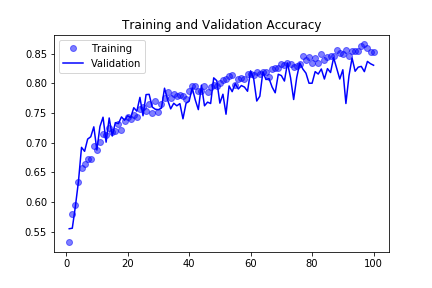
\includegraphics[width=\linewidth]{convnetFromScratch_Accuracy}
  \caption{Dogs vs. Cats Model Training Accuracy}
  \label{fig:CvDAcc}
\end{figure}

\begin{figure}[h]
  \centering
  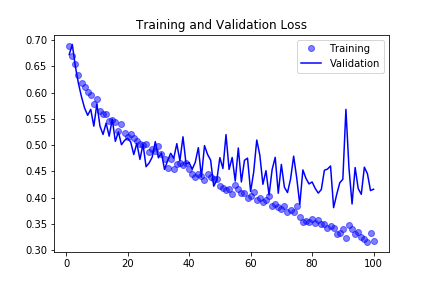
\includegraphics[width=\linewidth]{convnetFromScratch_Loss}
  \caption{Dogs vs. Cats Model Training Loss}
  \label{fig:CvDLoss}
\end{figure}

The Network was then trained on the augmented and preprocessed images for 100 epochs and achieves a final accuracy on the test images of 81\% (Fig.: \ref{fig:CvDAcc} \& \ref{fig:CvDLoss}).

While 81-82\% accuracy is not the best possible result, the network shows that training a network on a small but augmented dataset still shows an increase in accuracy of about 15\% relative to a network trained without augmenting the dataset.
Without increasing the dataset size the accuracy is likely limited to 86-87\% according to \cite{DLwP}.

\section{IntersectNet}
\subsection{Scope of Project}
The Network aims to solve a problem similar to the problem identified in \cite{IntersectNet} and \citep{E2ENavigation}.
However, by using spherical imaging it is suspected that the temporal component of the LCRN built in the paper can be circumvented.
This project tries to show that the use of equirectangular images can simplify the recognition of intersections.
The goal of this project is the creation of a network to recognize and classify indoor corridors and intersections.

\subsection{CG Dataset}
As there are no datasets of solely corridors and intersections that are taken at the correct height for a mobile robot, and are labelled correctly, a blender script is created to generate CG renders of corridor samples.

\begin{figure}[h]
  \centering
  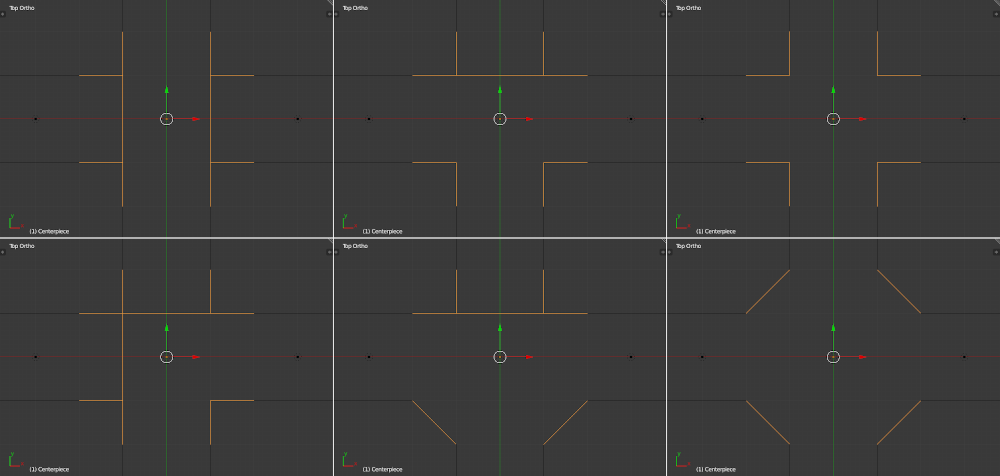
\includegraphics[width=\linewidth]{Blender_Schematic_Combined}
  \caption{Different Options for the Centerpiece}
  \label{fig:Centerpiece}
\end{figure}

The Script has a list of different centerpieces for the different amount of possible connections to adjacent corridors.
The scene is deemed a corridor, if it has two or less connections, resulting in a straight corridor, a corner, or a dead end.
If the centerpiece has three or four connections, it is considered an intersection.
Each intersection option has two different layouts, one with soft, and one with hard corners (Fig.: \ref{fig:Centerpiece}).
Additionally the centerpiece is rotated randomly in 90°-steps.
The script also uses a list of different Textures for floor, ceiling and walls to further randomize the scene.

\begin{figure}[h]
  \centering
  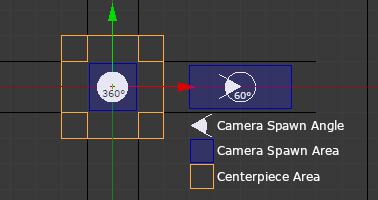
\includegraphics[width=\linewidth]{Blender_CamSpawnArea}
  \caption{Different Options for the camera Placement}
  \label{fig:Camspawn}
\end{figure}

After the layout is generated, the camera is placed semi-randomly (Fig.: \ref{fig:Camspawn}):
\begin{itemize}
\item For intersections the camera is placed within the intersection at a random rotation angle.
\item For corridors the camera is placed either inside the centerpiece or inside an adjacent corridor facing towards the intersection with a random variation of ±30°.
\end{itemize}

Finally the script renders normal and spherical images.
During renders of the test set both pictures are rendered together, so the test dataset contains the same layout in both perspectives with the same name (Fig.: \ref{fig:RenderSample}).

The generated dataset contains 18.000 images, 9.000 images in each perspective (normal and equirectangular).
These images are split into 5.000 training images, 2.000 validation images, and 2.000 test images.
Each split has an equal amount of corridor and intersection images.

\subsection{Network Structure and Training}
The network is structured into three convolutional layers, each followed by a pooling layer to abstract the features.
After the convolutional layers, the network has a layer to flatten the extracted information.
During training a 50\% dropout is used to counteract the limited variety of the dataset. Finally, two fully connected layers processes the information and produce the final prediction value.

\begin{figure}[h]
  \centering
  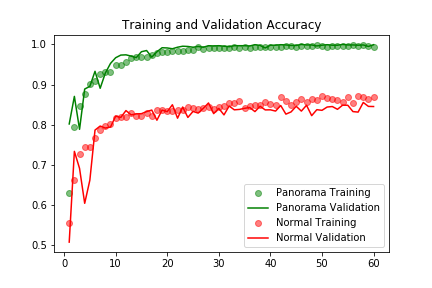
\includegraphics[width=\linewidth]{intersectNet_0831-0849_Accuracy}
  \caption{IntersectNet Accuracies}
  \label{fig:IntersectNetAcc}
\end{figure}

\begin{figure}[h]
  \centering
  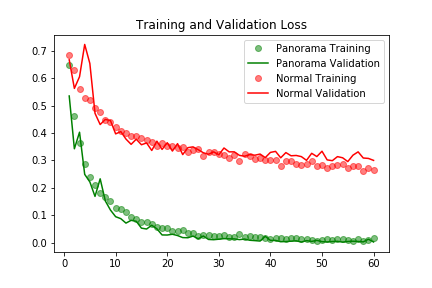
\includegraphics[width=\linewidth]{intersectNet_0831-0849_Loss}
  \caption{IntersectNet Losses}
  \label{fig:IntersectNetLoss}
\end{figure}

Two networks are trained, one with the normal perspective images, and one with the equirectangular images for comparison (Fig.: \ref{fig:IntersectNetAcc} \& \ref{fig:IntersectNetLoss}).
The training was conducted for 60 epochs, which took approximately 1 h 15 min.

\begin{table}[h]
  \caption{Accuracies and Losses of IntersectNet Models}
  \label{tab:IntersectNetAccLoss}
  \begin{tabular}{ c | r | l }
    \toprule
    Image Type & Accuracy & Loss \\
    \midrule
    Normal & 0,8420 & 0,3153 \\
	Spherical & 0,9999 & 0,0005 \\
  	\bottomrule
  \end{tabular}
\end{table}

The final results of both networks are shown in Table \ref{tab:IntersectNetAccLoss}.

\subsection{Test with Real Images}
To evaluate the ability of the network to distinguish real pictures of corridors and intersections, 30 images, 12 images of corridors and intersections each, as well as 6 images of locations hard to distinguish (lobby, outdoors, and staircase pictures).
However the network only predicts 14 of the 24 labelled pictures correctly (58\%).
All errors are corridors wrongly predicted as intersections, which means the network tends to classify pictures as intersections instead of corridors.
The reason for this inaccuracy is hard to judge, one possibility is the strong difference between corridors and intersections in the CG dataset, so the network might recognize wider corridors or open spaces as intersections as it learned that corridors are as narrow as the CG dataset suggests (~2 m wide corridors).
Another reason might be some bright light sources and reflections leading the network to assume additional paths, as the corridors in the dataset are only dimly lit.

\section{Results and Future Work}
While the network performs well on the CG images, it is insufficient for use on real images, likely reasons are the limited variety and quality of the CG dataset.
Nonetheless, the project shows the advantages of using spherical imaging for autonomous navigation and detection tasks.
The spherical images reduce the sensors needed for reliable detection and may also reduce the reliance of image sequences, at least for mobile robots in indoor environments.

To further prove these arguments, future work would focus on either improving the quality of the CG dataset, or gathering a dataset of real equirectangular images to properly train a network.
Additionally, the network can be implemented into a navigation system of a mobile robot to test the detection of intersections and allow navigation by simple instructions, i.e. "turn left at the next intersection", to simplify robot navigation in indoor corridor environments.

\begin{acks}
To Prof. Shigang Li, for the guidance and continuous help with research and reference material.

To Prof. Toshiharu Kosaku, for the help with setting up the workstation and the introduction to the mobile robot.
\end{acks}

\bibliographystyle{ACM-Reference-Format}
\bibliography{ProjectRep}

\appendix

\begin{figure*}[h]
  \centering
  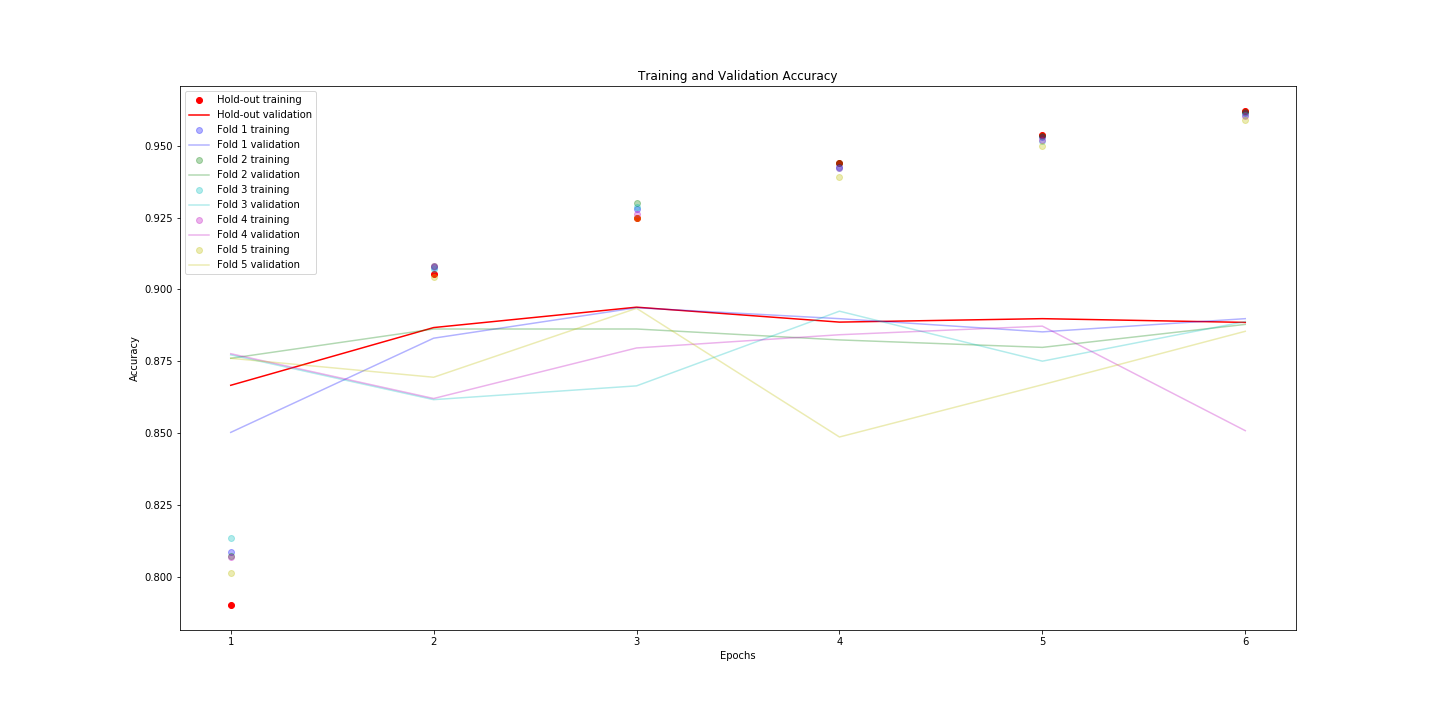
\includegraphics[width=\linewidth]{classifyMovieReviews_Accuracy}
  \caption{Movie Review Models Training Accuracies}
  \label{fig:MovieAcc}
\end{figure*}

\begin{figure*}[h]
  \centering
  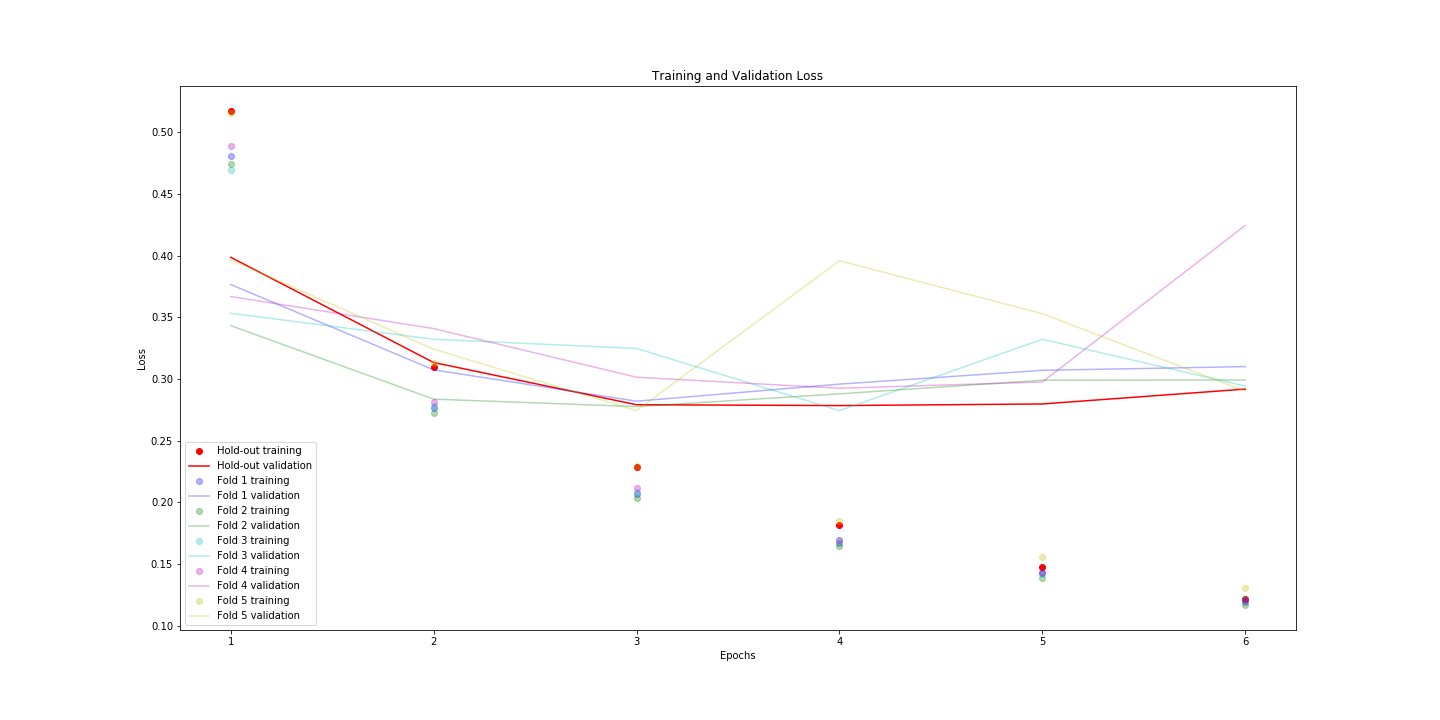
\includegraphics[width=\linewidth]{classifyMovieReviews_Loss}
  \caption{Movie Review Models Training Losses}
  \label{fig:MovieLoss}
\end{figure*}

\begin{figure*}[h]
  \centering
  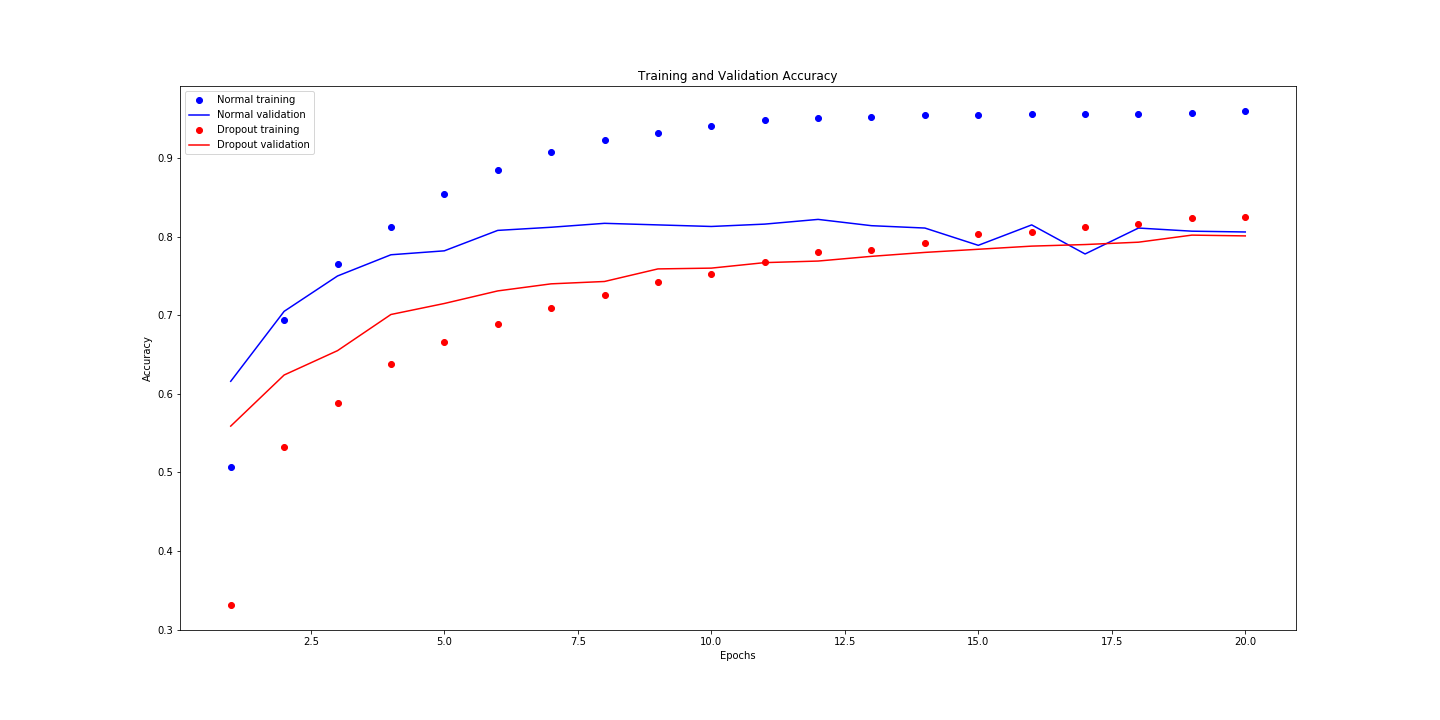
\includegraphics[width=\linewidth]{classifyNewswireTopics_Accuracy}
  \caption{Newswire Topics Models Training Accuracies}
  \label{fig:NewswireAcc}
\end{figure*}

\begin{figure*}[h]
  \centering
  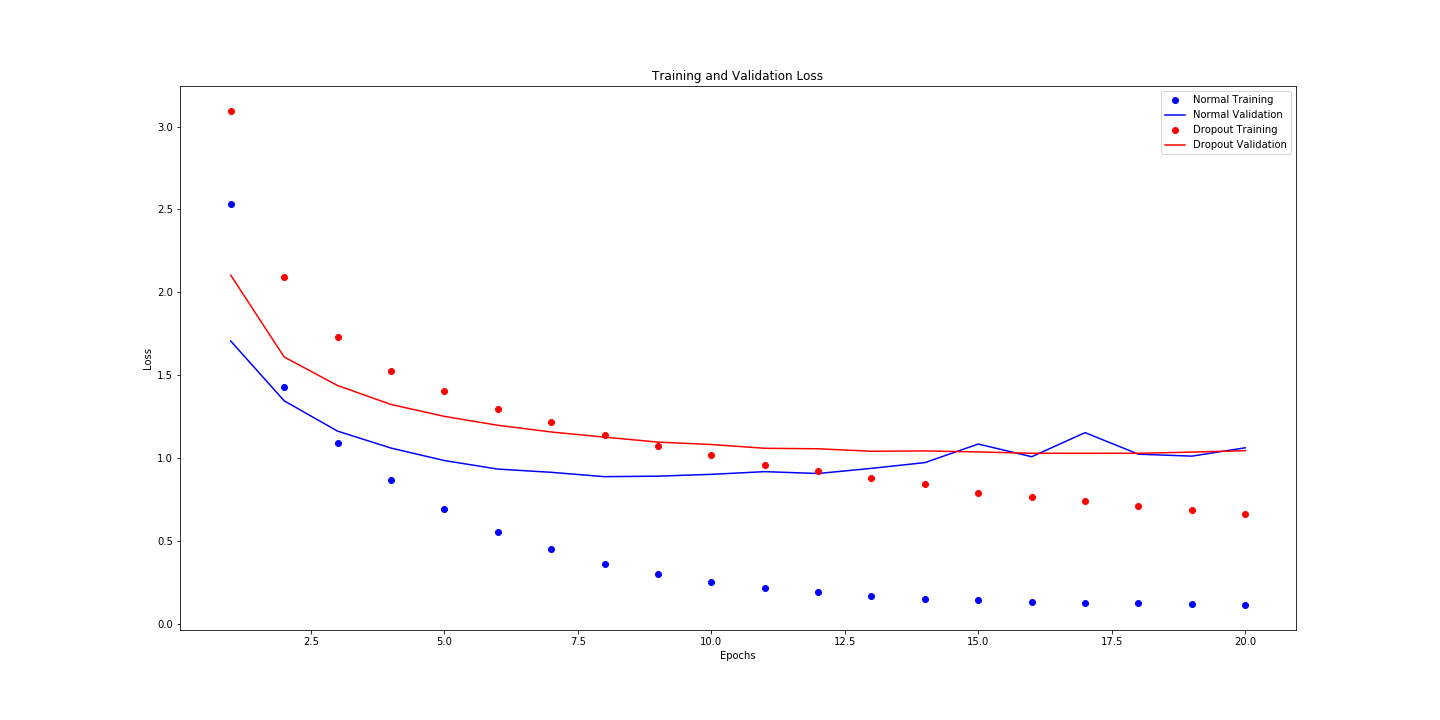
\includegraphics[width=\linewidth]{classifyNewswireTopics_Loss}
  \caption{Newswire Topics Models Training Losses}
  \label{fig:NewswireLoss}
\end{figure*}

\begin{figure*}[h]
  \centering
  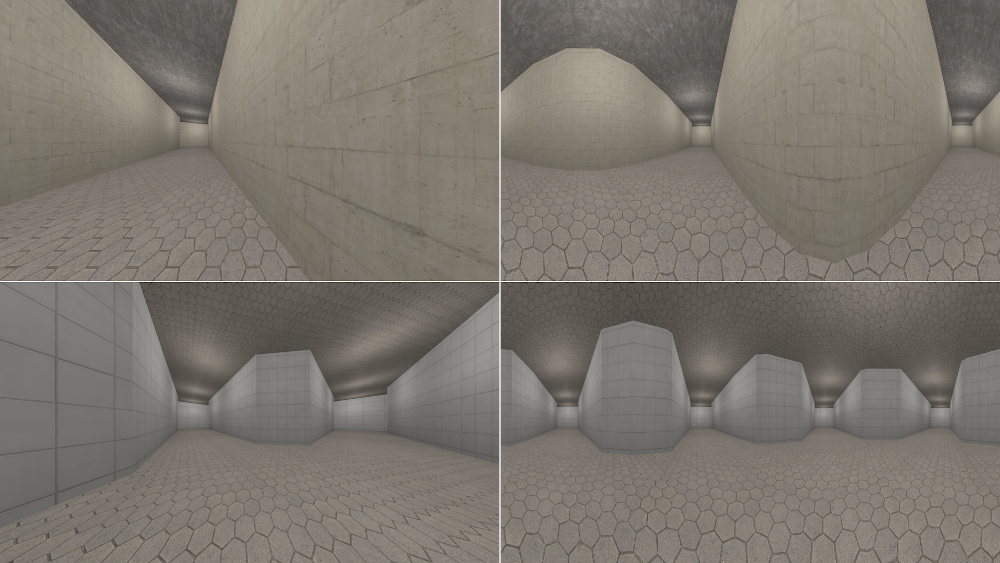
\includegraphics[width=\linewidth]{Blender_NormalPanoComparison}
  \caption{Rendered Test Images, Normal (left) and Spherical (right), Corridor (top) and Intersection (bottom)}
  \label{fig:RenderSample}
\end{figure*}

\end{document}
\endinput